\section{Results}
\label{sec:results}

\subsection{Contextual chunks versus reranking}
\label{sec:results-main}

Table~\ref{tab:retrieval} reports retrieval quality on the full set of 234
queries. Replacing flat chunks with contextualized chunks lifts recall@10 from
0.466 to 0.530 with BM25 fusion (arms \arm{a} and \arm{b}) and from 0.517 to
0.658 without it (arms \arm{e} and \arm{f}). The gain is wider on the dense-only
path, and arm~\arm{f} is the strongest configuration in the table on recall@10,
recall@50, document recall@10 and miss@50.

\begin{table}[t]
\centering
\small
\caption{Retrieval quality on the full set of 234 queries with gold chunks (3{,}134-chunk corpus, Apple~M2, MLX fp16). Metrics use gold groups: a hit on an overlapping neighboring window (within two positions) counts as the same text.}
\label{tab:retrieval}
\footnotesize
\begin{tabular}{lrrrrrrrr}
\toprule
Arm & R@1 & R@5 & R@10 & R@50 & MRR@10 & nDCG@10 & docR@10 & miss@50 \\
\midrule
A: flat, RRF & 0.107 & 0.333 & 0.466 & 0.752 & 0.207 & 0.268 & 0.568 & 0.248 \\
B: contextualized, RRF & 0.192 & 0.423 & 0.530 & 0.859 & 0.288 & 0.345 & 0.615 & 0.141 \\
E: flat, dense-only & 0.141 & 0.410 & 0.517 & 0.821 & 0.259 & 0.321 & 0.650 & 0.179 \\
\textbf{F: contextualized, dense-only} & 0.197 & 0.526 & 0.658 & 0.910 & 0.328 & 0.406 & 0.739 & 0.090 \\
G: distilled, dense-only & 0.218 & 0.517 & 0.620 & 0.897 & 0.342 & 0.409 & 0.709 & 0.103 \\
H: distilled, RRF & 0.197 & 0.414 & 0.530 & 0.863 & 0.288 & 0.345 & 0.632 & 0.137 \\
\bottomrule
\end{tabular}
\end{table}


A single reranked query costs about a minute, so arms \arm{c} and \arm{d} were
run on a subset of sixty queries. Every remaining arm was rerun on the same
subset, and Table~\ref{tab:rerank-subset} reports the result. The subset is a
fixed-seed random draw stratified by query type: fifteen queries of each type,
covering all five categories (14 IT, 14 security, 13 food, 11 pharmacy, 8
construction). Arm-to-arm comparisons hold, but the absolute values here differ
from the full set, where arms \arm{f} and \arm{g} reach 0.658 and 0.620.

Contextualization is the largest effect in the table, and it survives both
query paths: on the dense-only path recall@10 moves from 0.467 in arm~\arm{e} to
0.550 in arm~\arm{f}, on the fused path from 0.400 in arm~\arm{a} to 0.450 in
arm~\arm{b}, and over the full set the dense-only gain is wider still, from
0.517 to 0.658.

The reranker does improve the contextualized index, by an amount comparable to
contextualization itself, but the gain is not statistically resolved at sixty
queries. Recall@10 rises from 0.550 in arm~\arm{f} to 0.650 in arm~\arm{c}, a
paired difference of 0.100 with a 95\% bootstrap interval of $[0.000, 0.200]$;
against the distilled arm~\arm{g} the same comparison gives 0.050, with an
interval of $[-0.150, 0.050]$ for the difference arm~\arm{g} minus arm~\arm{c}.
Reaching 0.650 costs a median latency of 54{,}732~ms against 40.5~ms, a factor
of 1{,}351 over the contextualized dense-only arm.

Reranking flat chunks, in contrast, buys nothing. Arm~\arm{d} spends
43{,}383~ms per query to reach recall@10 of 0.467, which is exactly the value of
the dense-only flat arm~\arm{e} at 39.0~ms. A reranker can only reorder
candidates that the index already contains, and the missing document context is
not among them.

BM25 fusion contributes nothing on this corpus either. Arm~\arm{h} fuses the
distilled context with BM25 and reaches 0.450, the same value as arm~\arm{b} on
teacher context, so fusion pulls the distilled arm down from 0.600 in
arm~\arm{g} to 0.450 in arm~\arm{h}, a paired difference of 0.150 with a 95\%
interval of $[0.017, 0.283]$. Section~\ref{sec:ablations} shows that this is not
a question of tuning.

\begin{table}[t]
\centering
\small
\caption{All eight arms, measured on the same stratified subset of sixty queries (fifteen of each type, all five categories represented). Arm~\arm{g} reaches recall@10 of 0.600 at a median latency of 41~ms, and the reranked arm~\arm{c} reaches 0.650 at 54.7~s.}
\label{tab:rerank-subset}
\begin{tabular}{lrrrrr}
\toprule
Arm & R@1 & R@5 & R@10 & MRR@10 & nDCG@10 \\
\midrule
A: flat, RRF & 0.100 & 0.250 & 0.400 & 0.171 & 0.223 \\
B: contextualized, RRF & 0.150 & 0.350 & 0.450 & 0.233 & 0.284 \\
E: flat, dense-only & 0.033 & 0.350 & 0.467 & 0.177 & 0.247 \\
F: contextualized, dense-only & 0.167 & 0.433 & 0.550 & 0.265 & 0.332 \\
\textbf{G: distilled, dense-only} & 0.217 & 0.483 & 0.600 & 0.327 & 0.392 \\
H: distilled, RRF & 0.167 & 0.317 & 0.450 & 0.237 & 0.287 \\
C: contextualized, RRF, reranked & 0.183 & 0.517 & 0.650 & 0.339 & 0.414 \\
D: flat, RRF, reranked & 0.133 & 0.383 & 0.467 & 0.238 & 0.293 \\
\bottomrule
\end{tabular}
\end{table}


\begin{figure}[t]
\centering
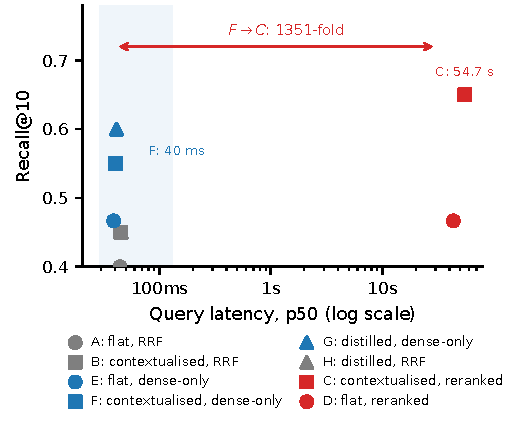
\includegraphics[width=0.62\linewidth]{figures/fig_quality_latency.pdf}
\caption{Quality against median latency, all eight arms on the same sixty
queries (logarithmic horizontal axis). The six reranker-free arms run in tens of
milliseconds; the two reranked arms run for about a minute.}
\label{fig:quality-latency}
\end{figure}

Latency is summarized in Table~\ref{tab:latency}. The reranker-free arms are
hard to tell apart in cost, 39.0 to 45.8~ms per query, of which 32 to 35~ms is
query encoding, while the reranked arms are three orders of magnitude slower. On
a single device that is roughly twenty-five queries per second against one query
per minute.

\begin{table}[t]
\centering
\small
\caption{Query latency (M2 GPU, MLX fp16, warmed). ``Total'' is the end-to-end retrieval call, including query encoding, BM25, fusion and, for arms \arm{c} and \arm{d}, reranking.}
\label{tab:latency}
\begin{tabular}{lrrr}
\toprule
Arm & p50 & p95 & encode \\
\midrule
A: flat, RRF & 44 & 64 & 32 \\
B: contextualized, RRF & 45 & 65 & 32 \\
E: flat, dense-only & 39 & 42 & 34 \\
\textbf{F: contextualized, dense-only} & 40 & 43 & 35 \\
G: distilled, dense-only & 41 & 46 & 35 \\
H: distilled, RRF & 46 & 65 & 32 \\
C: contextualized, RRF, reranked & 54732 & 71445 & 494 \\
D: flat, RRF, reranked & 43383 & 69291 & 365 \\
\bottomrule
\end{tabular}
\end{table}


\subsection{Distilled context on the target device}
\label{sec:results-distill}

Arm~\arm{g} uses contexts generated by the distilled 0.6B student in place of
the API teacher. On the full query set recall@10 falls from 0.658 to 0.620, a
paired difference of 0.038 with a 95\% bootstrap interval of $[-0.021, 0.098]$,
so the two are not distinguishable at this sample size, while MRR@10 and
nDCG@10 rise slightly, from 0.328 to 0.342 and from 0.406 to 0.409. On the
stratified subset the order reverses: the student reaches 0.600 against 0.550
for the teacher, a paired difference of 0.050 with an interval of
$[-0.050, 0.150]$. At this scale the two models are equivalent for retrieval,
and the student needs neither an API key nor a network at ingest time.

The student writes shorter contexts than the teacher, 263 characters against 295
on average, and the stratified analysis of Section~\ref{sec:strata} shows that
the brevity is not uniformly helpful.

Fused with BM25 the student context loses the entire gain: on the stratified
subset arm~\arm{h} reaches 0.450, exactly the value of arm~\arm{b} in the same
flat-versus-contextualized comparison, and on the full set both reach 0.530, so
the distilled context adds nothing once the sparse channel is fused. This is
consistent with the broader observation that the sparse channel is the weaker
component here.

Table~\ref{tab:ingest} gives the ingest comparison. The on-device path takes
4.49~h against 1.85~h for the API, a factor of 2.4, and costs nothing per run;
the prefix key/value cache is what keeps the difference tolerable, since without
it the prefill stage alone would need an estimated 7.08~h.

\begin{table}[t]
\centering
\small
\caption{Context-generation cost for the whole corpus (3{,}134 chunks, 82 documents, 24.3M prompt tokens): API teacher vs.\ distilled 0.6B model running on-device.}
\label{tab:ingest}
\begin{tabular}{lrr}
\toprule
 & Teacher (API) & Student (on-device) \\
\midrule
Model & \texttt{deepseek-v4.1-flash} & \texttt{Qwen3-0.6B} with LoRA \\
Wall-clock (h) & 1.85 & 4.49 \\
Per chunk, median (s) & 2.06 & 4.20 \\
Prefill (h) & -- & 2.31 \\
Decode (h) & -- & 2.19 \\
Output tokens (med./max) & -- & 90/160 \\
Cost (USD) & \textbf{\$0.82} & \textbf{\$0} \\
Data leaves device & yes & no \\
\bottomrule
\end{tabular}
\end{table}


\begin{figure}[t]
\centering
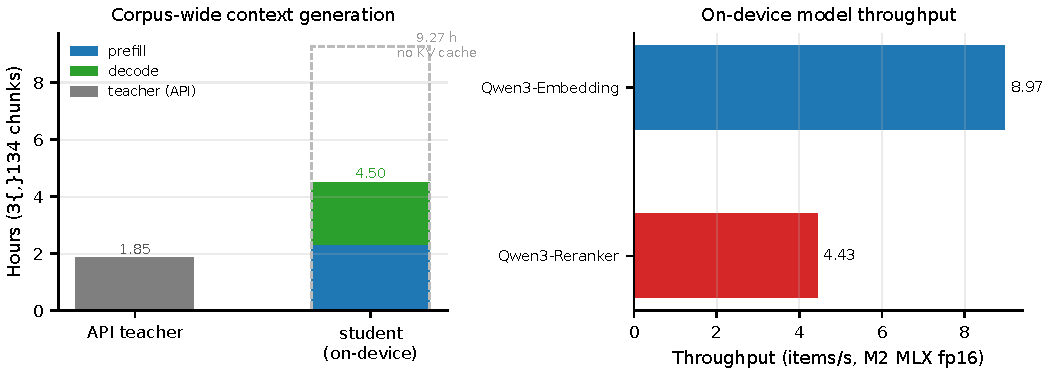
\includegraphics[width=\linewidth]{figures/fig_ingest.pdf}
\caption{Corpus-wide context generation (left) and query-time model throughput
(right). The dashed outline marks the estimated cost of the student without the
prefix key/value cache.}
\label{fig:ingest}
\end{figure}

\subsection{Ablations}
\label{sec:ablations}

Table~\ref{tab:ablations} collects the ablations, computed in memory over the
indexed vectors so that every variant sees identical candidate sets.

\paragraph{Embedding dimension.}
Truncating the 1{,}024-dimensional embeddings to 512 dimensions does not reduce
quality. With teacher context, recall@10 rises from 0.658 to 0.667 and miss@50
falls from 0.090 to 0.064; with student context, recall@10 rises from 0.615 to
0.641 and MRR@10 from 0.341 to 0.354. Truncation to 256 or 128 dimensions
degrades both relative to 512; for the teacher the two values sit close together
(0.568 against 0.573), though we did not run a paired test on those two.

\paragraph{Instruction language.}
Russian works as well as English for the query instruction. On teacher context
it is neutral on recall@10 and slightly better on MRR@10; on student context it
improves recall@10 from 0.615 to 0.650 and MRR@10 from 0.341 to 0.352. The two
levers also combine: truncation to 512 dimensions with a Russian instruction
gives the best student configuration in the table, recall@10 of 0.658 and
MRR@10 of 0.363, which matches the teacher baseline in recall@10 and exceeds it
in MRR@10 at half the vector size.

\paragraph{Fusion.}
No fusion setting recovers the loss caused by the sparse channel. BM25 alone
reaches recall@10 of 0.380 for the teacher context and 0.372 for the student
context, well below the dense-only values of 0.658 and 0.615. Lowering the rank
constant to one, the most favorable setting, still leaves fusion below
dense-only, and raising the weight of the dense channel to a ratio of one to
0.25 approaches but never reaches it. Deepening the BM25 channel from twenty to
two hundred candidates raises teacher recall monotonically from 0.508 to 0.538,
and neither arm reaches the dense-only value.

\begin{table}[t]
\centering
\small
\caption{Retrieval ablations computed in-memory on the indexed vectors (teacher arm F, student arm G; 234 queries, dense-only unless noted). $\Delta$ is student $-$ teacher.}
\label{tab:ablations}
\begin{tabular}{lrrrr}
\toprule
 & \multicolumn{2}{c}{Teacher (F)} & \multicolumn{2}{c}{Student (G)} \\
\cmidrule(lr){2-3}\cmidrule(lr){4-5}
Setting & R@10 & MRR@10 & R@10 & MRR@10 \\
\midrule
\multicolumn{5}{l}{\emph{MRL dimension}} \\
\quad 1024 & 0.658 & 0.328 & 0.615 & 0.341 \\
\quad 512 & 0.667 & 0.328 & 0.641 & 0.354 \\
\quad 256 & 0.568 & 0.303 & 0.611 & 0.332 \\
\quad 128 & 0.573 & 0.296 & 0.586 & 0.302 \\
\addlinespace[2pt]
\multicolumn{5}{l}{\emph{Query instruction}} \\
\quad English & 0.658 & 0.328 & 0.615 & 0.341 \\
\quad Russian & 0.658 & 0.331 & 0.650 & 0.352 \\
\addlinespace[2pt]
\multicolumn{5}{l}{\emph{Hybrid fusion (RRF)}} \\
\quad dense-only & 0.658 & 0.328 & 0.615 & 0.341 \\
\quad BM25-only & 0.380 & 0.189 & 0.372 & 0.184 \\
\quad $k{=}1$, 1:1 & 0.611 & 0.304 & 0.603 & 0.305 \\
\quad $k{=}10$, 1:1 & 0.581 & 0.295 & 0.607 & 0.292 \\
\quad $k{=}60$, 1:1 & 0.530 & 0.289 & 0.517 & 0.266 \\
\quad $k{=}60$, 1:0.25 & 0.645 & 0.314 & 0.603 & 0.297 \\
\addlinespace[2pt]
\multicolumn{5}{l}{\emph{Best combination}} \\
\quad d=512, Russian & 0.675 & 0.331 & 0.658 & 0.363 \\
\addlinespace[2pt]
\bottomrule
\end{tabular}
\end{table}


A stronger sparse backend does not change the picture. Table~\ref{tab:bm25}
compares the in-memory BM25Okapi implementation with the \texttt{Qdrant/bm25}
sparse backend, which applies IDF on the server side. The stronger backend
improves BM25-only recall@10 from 0.325 to 0.355 and hybrid recall@10 from 0.466
to 0.504 for flat chunks and from 0.530 to 0.556 for contextualized chunks, at
about fifty milliseconds per query, but it stays below the dense-only 0.658. On
a homogeneous corpus the sparse channel retrieves documents that share
vocabulary with the query yet do not answer it, and fusion carries that noise
into the dense ranking.

\begin{table}[t]
\centering
\small
\caption{BM25 backend comparison. \texttt{rank\_bm25} is an in-memory BM25Okapi with a Russian Snowball stemmer; \texttt{fastembed} uses \texttt{Qdrant/bm25} sparse vectors with IDF applied server-side (18 stop-word files, 92\,KB, no neural network). Hybrid columns are arms A/B.}
\label{tab:bm25}
\begin{tabular}{lrrrr}
\toprule
Setting & R@10 & MRR@10 & docR@10 & p50 (ms) \\
\midrule
\multicolumn{5}{l}{\emph{BM25-only}} \\
\quad \texttt{rank\_bm25} & 0.325 & 0.136 & 0.414 & 4.1 \\
\quad \texttt{fastembed} & 0.355 & 0.142 & 0.453 & 56.8 \\
\addlinespace[2pt]
\multicolumn{5}{l}{\emph{Hybrid RRF (dense and BM25)}} \\
\quad A flat, \texttt{rank\_bm25} & 0.466 & 0.207 & 0.568 & -- \\
\quad A flat, \texttt{fastembed} & 0.504 & 0.222 & 0.598 & -- \\
\quad B contextualized, \texttt{rank\_bm25} & 0.530 & 0.288 & 0.615 & -- \\
\quad B contextualized, \texttt{fastembed} & 0.556 & 0.286 & 0.645 & -- \\
\bottomrule
\end{tabular}
\end{table}


\subsection{Where distillation transfers}
\label{sec:strata}

Table~\ref{tab:strata} and Figure~\ref{fig:strata} break the teacher and student
arms down by query type, category and the kind of gold chunk.

The student context is the better of the two on multi-hop queries, where
recall@10 rises by 0.018 and MRR@10 by 0.038, and on the food category, where
recall@10 rises by 0.170. Both are settings in which a short context suffices:
multi-hop questions benefit from a concise statement that does not dilute the
connection between distant fragments, and the food documents are the most
template-like in the corpus.

The student is worse on semantic queries, where recall@10 falls by 0.125, and in
the IT, security and pharma categories, where the loss ranges from 0.106 to
0.130. These queries turn on exact details such as numbers, identifiers and
thresholds, and the student tends to generalize. The same pattern shows up in
the gold-chunk breakdown: tables are difficult for both models, with recall@10
between 0.483 and 0.540 against 0.694 to 0.728 on text, and the student loses
more ground on tables than on text.

\begin{table}[t]
\centering
\small
\caption{Per-stratum retrieval quality, teacher context (F) vs.\ student context (G); dense-only, 1024-d, English instruction. $\Delta$ is student $-$ teacher.}
\label{tab:strata}
\begin{tabular}{lrrrr}
\toprule
Stratum & $n$ & F R@10 & G R@10 & $\Delta$ R@10 \\
\midrule
\multicolumn{5}{l}{\emph{Query type}} \\
\quad lexical & 62 & 0.645 & 0.629 & -0.016 \\
\quad multihop & 57 & 0.684 & 0.702 & 0.018 \\
\quad semantic & 56 & 0.714 & 0.589 & -0.125 \\
\quad table & 59 & 0.593 & 0.542 & -0.051 \\
\addlinespace[2pt]
\multicolumn{5}{l}{\emph{Category}} \\
\quad construction & 35 & 0.486 & 0.486 & 0.000 \\
\quad food & 47 & 0.638 & 0.808 & 0.170 \\
\quad it & 59 & 0.712 & 0.593 & -0.119 \\
\quad pharma & 47 & 0.766 & 0.660 & -0.106 \\
\quad security & 46 & 0.630 & 0.500 & -0.130 \\
\addlinespace[2pt]
\multicolumn{5}{l}{\emph{Gold chunk}} \\
\quad gold table & 87 & 0.540 & 0.483 & -0.057 \\
\quad gold text & 147 & 0.728 & 0.694 & -0.034 \\
\addlinespace[2pt]
\bottomrule
\end{tabular}
\end{table}


\begin{figure}[t]
\centering
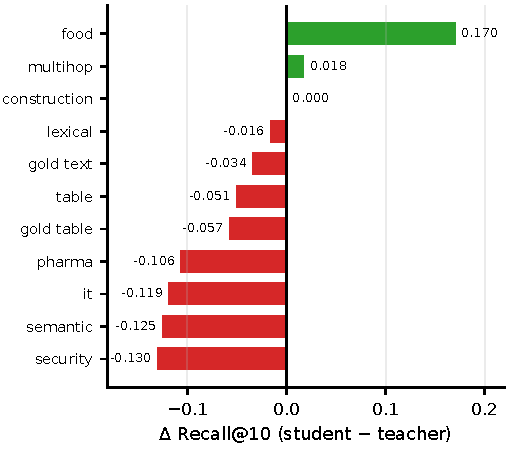
\includegraphics[width=0.60\linewidth]{figures/fig_strata.pdf}
\caption{Change in recall@10 when the teacher context is replaced by the
distilled context, by stratum.}
\label{fig:strata}
\end{figure}

\subsection{Cost and break-even}
\label{sec:breakeven}

The two pipelines differ in where their cost sits. Context generation costs 3.3
minutes per document on the device and 1.4 minutes per document through the API,
and it is paid once per document. Query processing costs 40~ms per query without
the reranker and 54.7~s with it, paid once per query. Writing
$T(D, Q) = D\,t_{\mathrm{ingest}} + Q\,t_{\mathrm{query}}$ for a corpus of $D$
documents and $Q$ queries, the reranker is never worth its query cost at a
practical workload: at $D = 500$ and $Q = 1{,}000$ the on-device reranker-free
pipeline needs 27.4 hours and the API pipeline 11.3 hours for USD~4.98, while
adding the reranker raises these to 42.6 and 26.5 hours respectively.

\begin{figure}[t]
\centering
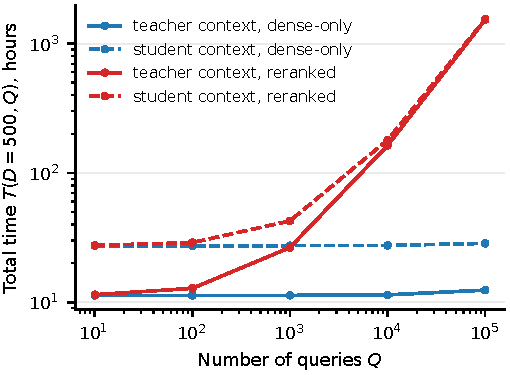
\includegraphics[width=0.62\linewidth]{figures/fig_breakeven.pdf}
\caption{Total time as a function of the number of queries for a corpus of 500
documents. The reranked configurations grow with the query count; the
reranker-free configurations are dominated by ingest.}
\label{fig:breakeven}
\end{figure}

The break-even between the two context generators lies in the ingest cost: the
API saves 2.6 hours per eighty-two documents and costs USD~0.82, while the
on-device path costs nothing and keeps the documents local. The API is
preferable when the corpus is generated once and hardware is the bottleneck;
the on-device path is preferable when the corpus is regenerated, when the
documents are sensitive, or when the device is the only hardware available.
